\documentclass[12pt, a4]{article}
\usepackage[margin=2cm]{geometry}
\usepackage{parskip}
\usepackage{nameref}
\usepackage{enumitem}
\usepackage{booktabs}
\usepackage{tabularx}
\usepackage{hyperref}
\usepackage[tiny]{titlesec}

\usepackage{amsmath}
\usepackage{amssymb}

\usepackage{fancyhdr}
\usepackage{titling}

\usepackage{pgfplots}
\pgfplotsset{compat=1.16}
\usetikzlibrary{decorations.pathreplacing,positioning, shapes,arrows,chains}


\usepackage{xcolor}
\usepackage{graphicx}
\usepackage{fancyvrb}
\usepackage{listings}
\usepackage{bm}
\usepackage{xcolor}
\usepackage{optidef}

\usepackage{pifont} % for cmark and xmark
\newcommand{\cmark}{\ding{51}}%
\newcommand{\xmark}{\ding{55}}%
\newcommand{\checkedbox}{\rlap{$\square$}{\raisebox{2pt}{\hspace{1pt}\cmark}}}
%\newcommand{\crossedBox}{\rlap{$\square$}{\large\hspace{1pt}\xmark}}


\xdefinecolor{gray}{rgb}{0.4,0.4,0.4}
\xdefinecolor{blue}{RGB}{58,95,205}
\xdefinecolor{darkgreen}{RGB}{0,100,0}

\newcommand{\lightgray}{black!30}

\newcommand{\plotDomain}{-1:8}

\newcommand{\addPlotLDownCoords}[1]{
	\addplot[mark=none, domain=\plotDomain, color=\lightgray,
	decoration={border,segment length=1mm,amplitude=1.5mm,angle=-135},
	postaction={decorate}
	] coordinates {#1};
	\addplot[mark=none, domain=\plotDomain] coordinates {#1};
}

\newcommand{\addPlotLDown}[1]{
	\addplot[mark=none, domain=\plotDomain, color=\lightgray,
	decoration={border,segment length=1mm,amplitude=1.5mm,angle=-135},
	postaction={decorate}
	] {#1};
	\addplot[mark=none, domain=\plotDomain] {#1};
}

\newcommand{\addPlotRUpCoords}[1]{
	\addplot[mark=none, domain=\plotDomain, color=\lightgray,
	decoration={border,segment length=1mm,amplitude=1.5mm,angle=135},
	postaction={decorate}
	] coordinates {#1};
	\addplot[mark=none, domain=\plotDomain] coordinates {#1};
}

\newcommand{\addPlotRUp}[1]{
	\addplot[mark=none, domain=\plotDomain, color=\lightgray,
	decoration={border,segment length=1mm,amplitude=1.5mm,angle=135},
	postaction={decorate}
	] {#1};
	\addplot[mark=none, domain=\plotDomain] {#1};
}

\lstset{% setup listings
	language=R,% set programming language
	basicstyle=\ttfamily\small,% basic font style
	keywordstyle=\color{blue},% keyword style
	commentstyle=\color{gray},% comment style
	numbers=left,% display line numbers on the left side
	numberstyle=\scriptsize,% use small line numbers
	numbersep=10pt,% space between line numbers and code
	tabsize=3,% sizes of tabs
	showstringspaces=false,% do not replace spaces in strings by a certain character
	captionpos=b,% positioning of the caption below
	breaklines=true,% automatic line breaking
	escapeinside={(*}{*)},% escaping to LaTeX
	fancyvrb=true,% verbatim code is typset by listings
	extendedchars=false,% prohibit extended chars (chars of codes 128--255)
	literate={"}{{\texttt{"}}}1{<-}{{$\bm\leftarrow$}}1{<<-}{{$\bm\twoheadleftarrow$}}1
	{~}{{$\bm\sim$}}1{<=}{{$\bm\le$}}1{>=}{{$\bm\ge$}}1{!=}{{$\bm\neq$}}1{^}{{$^{\bm\wedge}$}}1,% item to replace, text, length of chars
	alsoletter={.<-},% becomes a letter
	alsoother={$},% becomes other
	otherkeywords={!=, ~, $, \&, \%/\%, \%*\%, \%\%, <-, <<-, /},% other keywords
	deletekeywords={c}% remove keywords
}



\author{Pascal Lüscher}
\title{Mathematical Optimization – Problem set 7}

\makeatletter
\let\mytitle\@title
\makeatother

\pagestyle{fancy}
\fancyhf{}
\rhead{
	\mytitle\\
	\theauthor
}

\rfoot{
	Page: \thepage
}

\renewcommand{\arraystretch}{1.2} % more space in tables
\renewcommand\thesubsection{\thesection.\alph{subsection}}
\titleformat{\section}[hang]{\normalfont\bfseries\itshape}{\textup{\thesubsection}}{1em}{}

\titleformat{\subsection}[hang]{\normalsize\itshape}{\textup{\thesubsection}}{1em}{}[]

\newcommand{\norm}[1]{\lvert #1 \rvert}

\newcolumntype{L}{>{$}l<{$}} % math-mode version of "l" column type
\newcolumntype{R}{>{$}r<{$}} % math-mode version of "l" column type
\newcolumntype{C}{>{$}c<{$}} % math-mode version of "l" column type

\begin{document}
\section{Problem 1: The algorithm of Ford-Fulkerson and the value of a flow}
\begin{figure}[h]
	\centering
	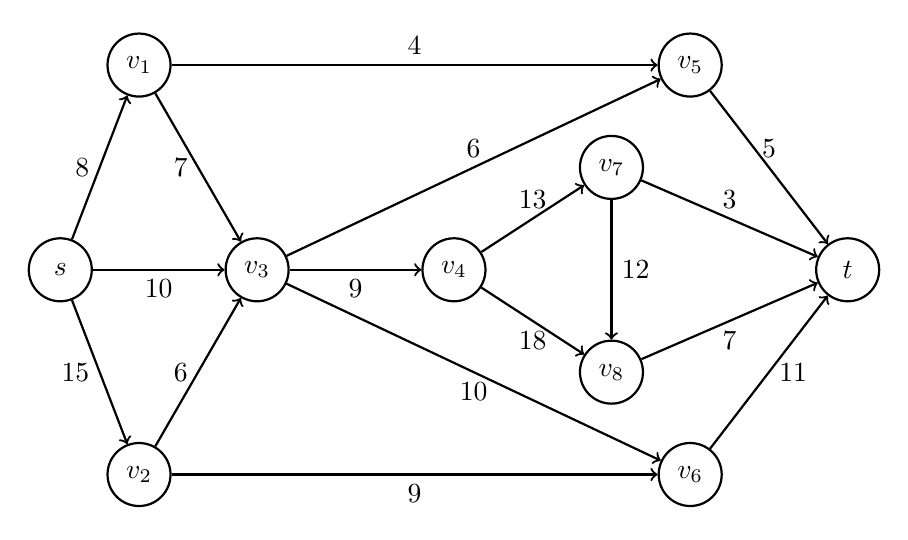
\begin{tikzpicture}[x=2cm, y=1.3cm]
		\begin{scope}[every node/.style={circle,thick,draw, minimum size=8mm}]
			\node (s) at (0,0) {$s$};
			\node (v1) at (0.5,2) {$v_1$};
			\node (v2) at (0.5,-2) {$v_2$};			
			\node (v3) at (1.25,0) {$v_3$};
			\node (v4) at (2.5,0) {$v_4$};
			\node (v5) at (4,2) {$v_5$};
			\node (v6) at (4,-2) {$v_6$};
			\node (v7) at (3.5,1) {$v_7$};
			\node (v8) at (3.5,-1) {$v_8$};
			\node (t) at (5,0) {$t$};
		\end{scope}
		\begin{scope}[every path/.style={thick,->}]
			\path (s)  
				edge node[left] {8} (v1)
				edge node[left] {15} (v2)
				edge node[below] {10} (v3);
			\path (v1)
				edge node[left] {7} (v3)
				edge node[above] {4} (v5);
			\path (v2)
				edge node[left] {6} (v3)
				edge node[below] {9} (v6);
			\path (v3)
				edge node[above] {6} (v5)
				edge node[below] {9} (v4)
				edge node[below] {10} (v6);
			\path (v4)
				edge node[above] {13} (v7)
				edge node[below] {18} (v8);
			\path (v5)
				edge node[above] {5} (t);
			\path (v6)
				edge node[right] {11} (t);
			\path (v7) 
				edge node[right] {12} (v8)
				edge node[above] {3} (t);
			\path (v8) 
				edge node[below] {7} (t);
		\end{scope}
	\end{tikzpicture}
	\caption{A digraph $G=(V,A)$ with edge capacities $u : A \rightarrow\mathbb{Z}_{\geq0}$}
	\label{fig:graph_prob_1}
\end{figure}
\subsection{Consider the graph $G=(V,A)$ with edge capacities $u : A \rightarrow\mathbb{Z}_{\geq0}$ given in \autoref{fig:graph_prob_1}. Apply the algorithm of Ford and Fulkerson to obtain a maximal $s$-$t$ flow. In every iteration, provide the current flow and its value, the corresponding residual graph, as well as an augmenting $s$-$t$ path together with its increment value $\gamma$ (or a certificate that there is no augmenting $s$-$t$ path).}
\begin{minipage}{.8\textwidth}
	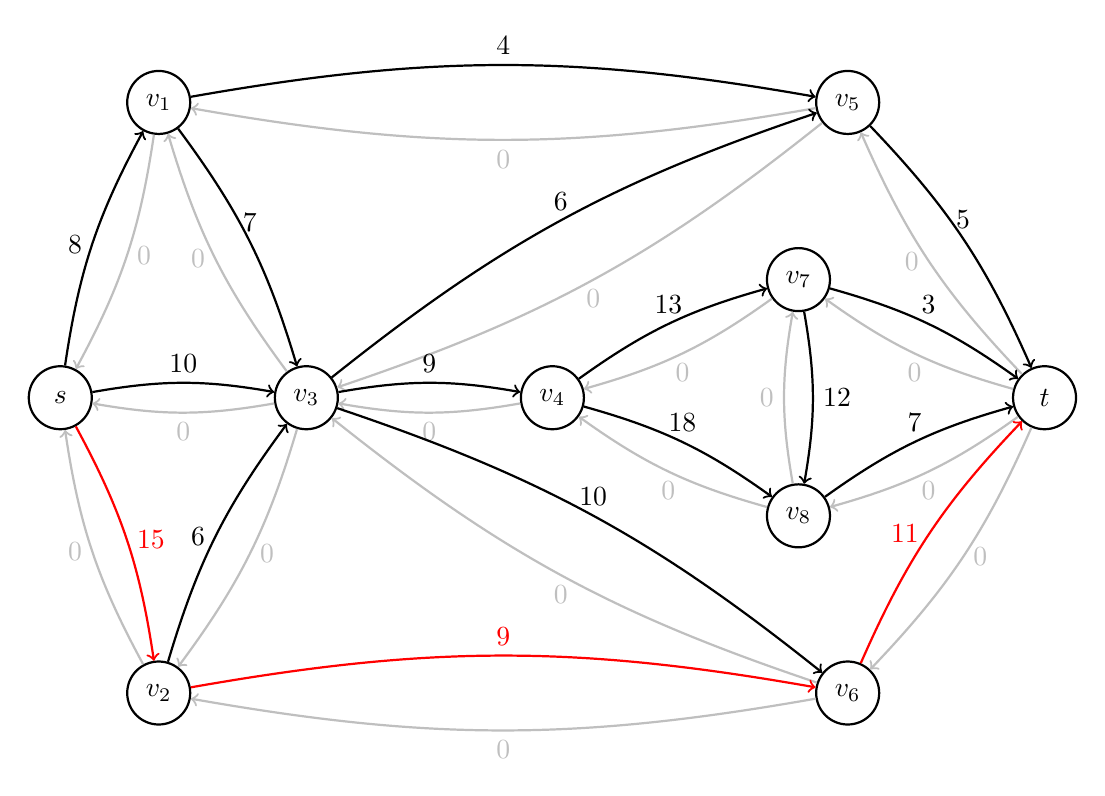
\begin{tikzpicture}[x=2.5cm, y=1.5cm]
		\begin{scope}[every node/.style={circle,thick,draw, minimum size=8mm}]
			\node (s) at (0,0) {$s$};
			\node (v1) at (0.5,2.5) {$v_1$};
			\node (v2) at (0.5,-2.5) {$v_2$};			
			\node (v3) at (1.25,0) {$v_3$};
			\node (v4) at (2.5,0) {$v_4$};
			\node (v5) at (4,2.5) {$v_5$};
			\node (v6) at (4,-2.5) {$v_6$};
			\node (v7) at (3.75,1) {$v_7$};
			\node (v8) at (3.75,-1) {$v_8$};
			\node (t) at (5,0) {$t$};
		\end{scope}
		\begin{scope}[every path/.style={thick,<-,bend right=10}]
			\path[lightgray] (s)  
				edge node[right] {0} (v1)
				edge node[left] {0} (v2)
				edge node[below] {0} (v3);
			\path[lightgray] (v1)
				edge node[left] {0} (v3)
				edge node[below] {0} (v5);
			\path[lightgray] (v2)
				edge node[right] {0} (v3)
				edge node[below] {0} (v6);
			\path[lightgray] (v3)
				edge node[below] {0} (v5)
				edge node[below] {0} (v4)
				edge node[below] {0} (v6);
			\path[lightgray] (v4)
				edge node[below] {0} (v7)
				edge node[below] {0} (v8);
			\path[lightgray] (v5)
				edge node[left] {0} (t);
			\path[lightgray] (v6)
				edge node[right] {0} (t);	
			\path[lightgray] (v7) 
				edge node[left] {0} (v8)
				edge node[below] {0} (t);
			\path[lightgray] (v8) 
				edge node[below] {0} (t);							
		\end{scope}
		\begin{scope}[every path/.style={thick,->, bend left=10}]
			\path (s)  
			edge node[left] {8} (v1)
			edge[red] node[right, red] {15} (v2)
			edge node[above] {10} (v3);
	
			\path (v1)
				edge node[above] {7} (v3)
				edge node[above] {4} (v5);
			\path (v2)
				edge node[left] {6} (v3)
				edge[red] node[above,red] {9} (v6);
			\path (v3)
				edge node[above] {6} (v5)
				edge node[above] {9} (v4)
				edge node[above] {10} (v6);
			\path (v4)
				edge node[above] {13} (v7)
				edge node[above] {18} (v8);
			\path (v5)
				edge node[above] {5} (t);
			\path (v6)
				edge[red] node[left,red] {11} (t);
			\path (v7) 
				edge node[right] {12} (v8)
				edge node[above] {3} (t);
			\path (v8) 
				edge node[above] {7} (t);
		\end{scope}
	\end{tikzpicture}
\end{minipage}
\begin{minipage}{.2\textwidth}
	\begin{tabular}{rr}
		\toprule
		what & value \\ \midrule
		$f$ & 0 \\
		{\color{red}$\gamma$} & 9 \\
		\bottomrule
	\end{tabular}
\end{minipage}


\begin{minipage}{.8\textwidth}
	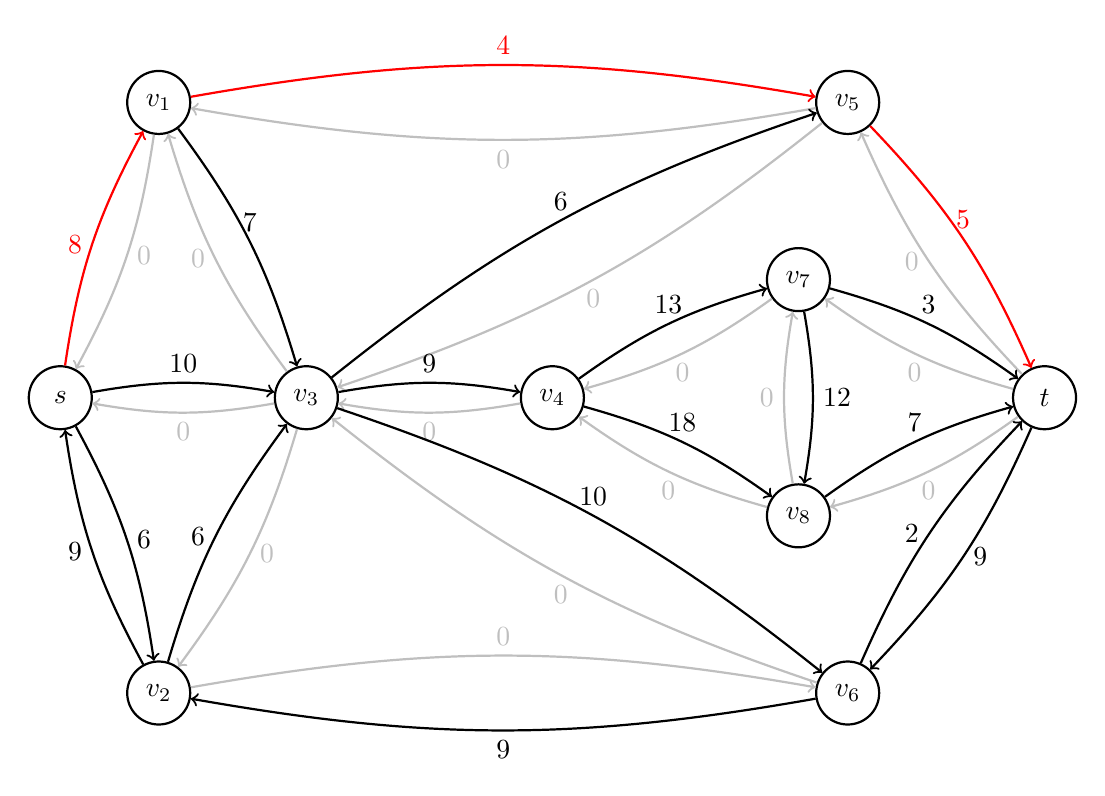
\begin{tikzpicture}[x=2.5cm, y=1.5cm]
		\begin{scope}[every node/.style={circle,thick,draw, minimum size=8mm}]
			\node (s) at (0,0) {$s$};
			\node (v1) at (0.5,2.5) {$v_1$};
			\node (v2) at (0.5,-2.5) {$v_2$};			
			\node (v3) at (1.25,0) {$v_3$};
			\node (v4) at (2.5,0) {$v_4$};
			\node (v5) at (4,2.5) {$v_5$};
			\node (v6) at (4,-2.5) {$v_6$};
			\node (v7) at (3.75,1) {$v_7$};
			\node (v8) at (3.75,-1) {$v_8$};
			\node (t) at (5,0) {$t$};
		\end{scope}
		\begin{scope}[every path/.style={thick,<-,bend right=10}]
			\path (s)  
			edge [lightgray] node[right] {0} (v1)
			edge node[left] {9} (v2)
			edge [lightgray] node[below] {0} (v3);
			\path[lightgray] (v1)
			edge node[left] {0} (v3)
			edge node[below] {0} (v5);
			\path (v2)
			edge [lightgray] node[right] {0} (v3)
			edge node[below] {9} (v6);
			\path[lightgray] (v3)
			edge node[below] {0} (v5)
			edge node[below] {0} (v4)
			edge node[below] {0} (v6);
			\path[lightgray] (v4)
			edge node[below] {0} (v7)
			edge node[below] {0} (v8);
			\path[lightgray] (v5)
			edge node[left] {0} (t);
			\path (v6)
			edge node[right] {9} (t);	
			\path[lightgray] (v7) 
			edge node[left] {0} (v8)
			edge node[below] {0} (t);
			\path[lightgray] (v8) 
			edge node[below] {0} (t);							
		\end{scope}
		\begin{scope}[every path/.style={thick,->, bend left=10}]
			\path (s)  
			edge [red] node[left] {8} (v1)
			edge node[right] {6} (v2)
			edge node[above] {10} (v3);
			
			\path (v1)
			edge node[above] {7} (v3)
			edge [red] node[above] {4} (v5);
			\path (v2)
			edge node[left] {6} (v3)
			edge [lightgray] node[above] {0} (v6);
			\path (v3)
			edge node[above] {6} (v5)
			edge node[above] {9} (v4)
			edge node[above] {10} (v6);
			\path (v4)
			edge node[above] {13} (v7)
			edge node[above] {18} (v8);
			\path (v5)
			edge [red] node[above] {5} (t);
			\path (v6)
			edge node[left] {2} (t);
			\path (v7) 
			edge node[right] {12} (v8)
			edge node[above] {3} (t);
			\path (v8) 
			edge node[above] {7} (t);
		\end{scope}
	\end{tikzpicture}
\end{minipage}
\begin{minipage}{.2\textwidth}
	\begin{tabular}{rr}
		\toprule
		what & value \\ \midrule
		$f$ & 9 \\
		{\color{red}$\gamma$} & 4 \\
		\bottomrule
	\end{tabular}
\end{minipage}


\begin{minipage}{.8\textwidth}
	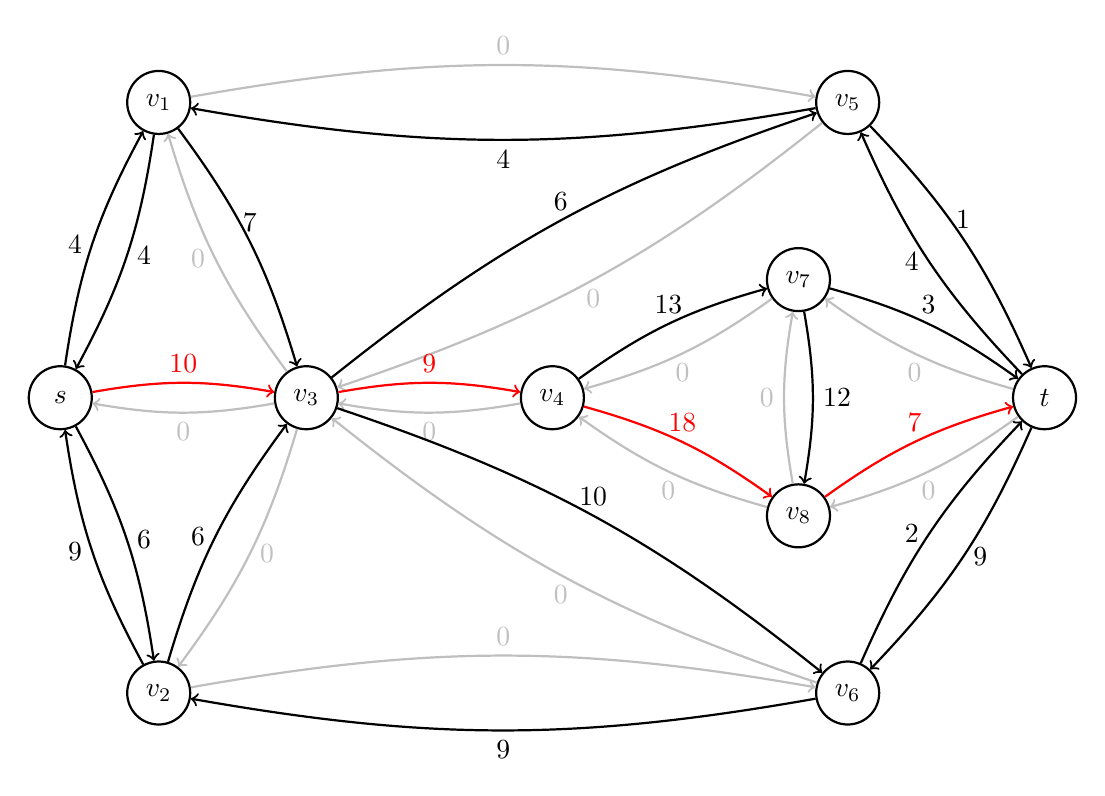
\begin{tikzpicture}[x=2.5cm, y=1.5cm]
		\begin{scope}[every node/.style={circle,thick,draw, minimum size=8mm}]
			\node (s) at (0,0) {$s$};
			\node (v1) at (0.5,2.5) {$v_1$};
			\node (v2) at (0.5,-2.5) {$v_2$};			
			\node (v3) at (1.25,0) {$v_3$};
			\node (v4) at (2.5,0) {$v_4$};
			\node (v5) at (4,2.5) {$v_5$};
			\node (v6) at (4,-2.5) {$v_6$};
			\node (v7) at (3.75,1) {$v_7$};
			\node (v8) at (3.75,-1) {$v_8$};
			\node (t) at (5,0) {$t$};
		\end{scope}
		\begin{scope}[every path/.style={thick,<-,bend right=10}]
			\path (s)  
			edge node[right] {4} (v1)
			edge node[left] {9} (v2)
			edge [lightgray] node[below] {0} (v3);
			\path (v1)
			edge[lightgray] node[left] {0} (v3)
			edge node[below] {4} (v5);
			\path (v2)
			edge [lightgray] node[right] {0} (v3)
			edge node[below] {9} (v6);
			\path[lightgray] (v3)
			edge node[below] {0} (v5)
			edge node[below] {0} (v4)
			edge node[below] {0} (v6);
			\path[lightgray] (v4)
			edge node[below] {0} (v7)
			edge node[below] {0} (v8);
			\path (v5)
			edge node[left] {4} (t);
			\path (v6)
			edge node[right] {9} (t);	
			\path[lightgray] (v7) 
			edge node[left] {0} (v8)
			edge node[below] {0} (t);
			\path[lightgray] (v8) 
			edge node[below] {0} (t);							
		\end{scope}
		\begin{scope}[every path/.style={thick,->, bend left=10}]
			\path (s)  
			edge node[left] {4} (v1)
			edge node[right] {6} (v2)
			edge [red] node[above] {10} (v3);
			
			\path (v1)
			edge node[above] {7} (v3)
			edge [lightgray] node[above] {0} (v5);
			\path (v2)
			edge node[left] {6} (v3)
			edge [lightgray] node[above] {0} (v6);
			\path (v3)
			edge node[above] {6} (v5)
			edge [red] node[above] {9} (v4)
			edge node[above] {10} (v6);
			\path (v4)
			edge node[above] {13} (v7)
			edge [red] node[above] {18} (v8);
			\path (v5)
			edge node[above] {1} (t);
			\path (v6)
			edge node[left] {2} (t);
			\path (v7) 
			edge node[right] {12} (v8)
			edge node[above] {3} (t);
			\path (v8) 
			edge [red] node[above] {7} (t);
		\end{scope}
	\end{tikzpicture}
\end{minipage}
\begin{minipage}{.2\textwidth}
	\begin{tabular}{rr}
		\toprule
		what & value \\ \midrule
		$f$ & 13 \\
		{\color{red}$\gamma$} & 7 \\
		\bottomrule
	\end{tabular}
\end{minipage}

\begin{minipage}{.8\textwidth}
	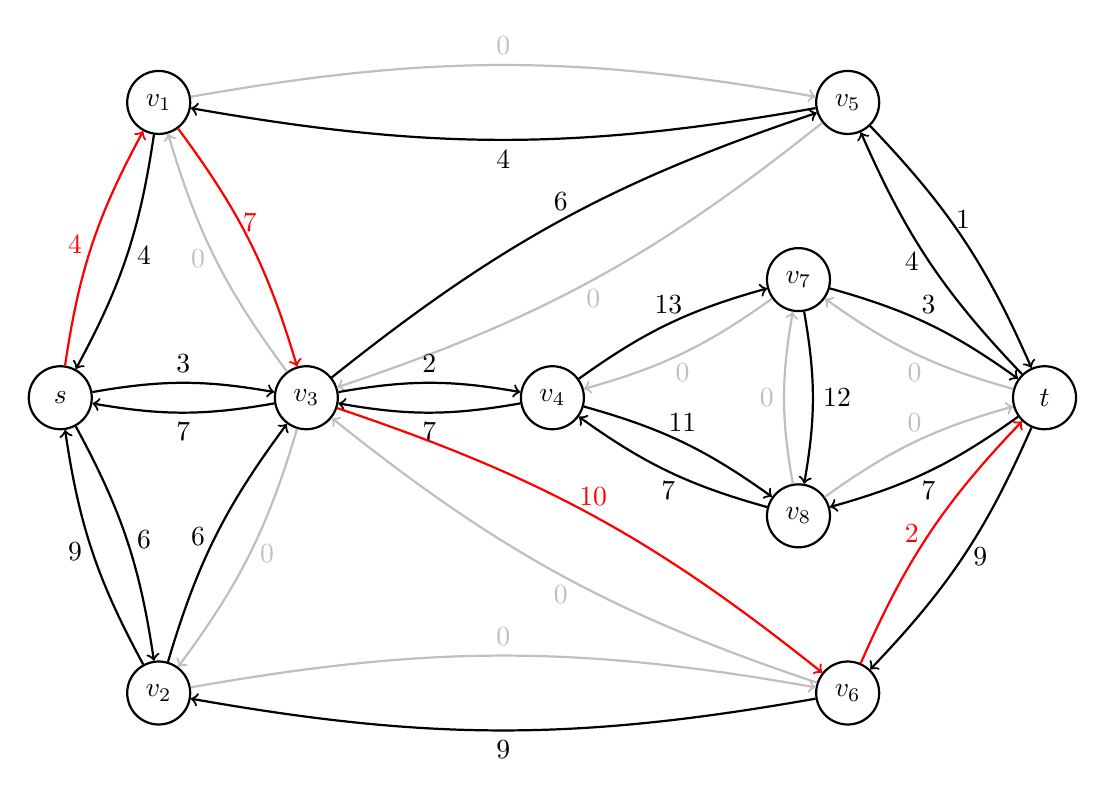
\begin{tikzpicture}[x=2.5cm, y=1.5cm]
		\begin{scope}[every node/.style={circle,thick,draw, minimum size=8mm}]
			\node (s) at (0,0) {$s$};
			\node (v1) at (0.5,2.5) {$v_1$};
			\node (v2) at (0.5,-2.5) {$v_2$};			
			\node (v3) at (1.25,0) {$v_3$};
			\node (v4) at (2.5,0) {$v_4$};
			\node (v5) at (4,2.5) {$v_5$};
			\node (v6) at (4,-2.5) {$v_6$};
			\node (v7) at (3.75,1) {$v_7$};
			\node (v8) at (3.75,-1) {$v_8$};
			\node (t) at (5,0) {$t$};
		\end{scope}
		\begin{scope}[every path/.style={thick,<-,bend right=10}]
			\path (s)  
			edge node[right] {4} (v1)
			edge node[left] {9} (v2)
			edge node[below] {7} (v3);
			\path (v1)
			edge [lightgray] node[left] {0} (v3)
			edge node[below] {4} (v5);
			\path (v2)
			edge [lightgray] node[right] {0} (v3)
			edge node[below] {9} (v6);
			\path (v3)
			edge [lightgray] node[below] {0} (v5)
			edge node[below] {7} (v4)
			edge [lightgray] node[below] {0} (v6);
			\path(v4)
			edge [lightgray] node[below] {0} (v7)
			edge node[below] {7} (v8);
			\path (v5)
			edge node[left] {4} (t);
			\path (v6)
			edge node[right] {9} (t);	
			\path[lightgray] (v7) 
			edge node[left] {0} (v8)
			edge node[below] {0} (t);
			\path (v8) 
			edge node[below] {7} (t);							
		\end{scope}
		\begin{scope}[every path/.style={thick,->, bend left=10}]
			\path (s)  
			edge [red] node[left] {4} (v1)
			edge node[right] {6} (v2)
			edge node[above] {3} (v3);
			
			\path (v1)
			edge [red] node[above] {7} (v3)
			edge [lightgray] node[above] {0} (v5);
			\path (v2)
			edge node[left] {6} (v3)
			edge [lightgray] node[above] {0} (v6);
			\path (v3)
			edge node[above] {6} (v5)
			edge node[above] {2} (v4)
			edge [red] node[above] {10} (v6);
			\path (v4)
			edge node[above] {13} (v7)
			edge node[above] {11} (v8);
			\path (v5)
			edge node[above] {1} (t);
			\path (v6)
			edge [red] node[left] {2} (t);
			\path (v7) 
			edge node[right] {12} (v8)
			edge node[above] {3} (t);
			\path (v8) 
			edge [lightgray] node[above] {0} (t);
		\end{scope}
	\end{tikzpicture}
\end{minipage}
\begin{minipage}{.2\textwidth}
	\begin{tabular}{rr}
		\toprule
		what & value \\ \midrule
		$f$ & 20 \\
		{\color{red}$\gamma$} & 2 \\
		\bottomrule
	\end{tabular}
\end{minipage}

\begin{minipage}{.8\textwidth}
	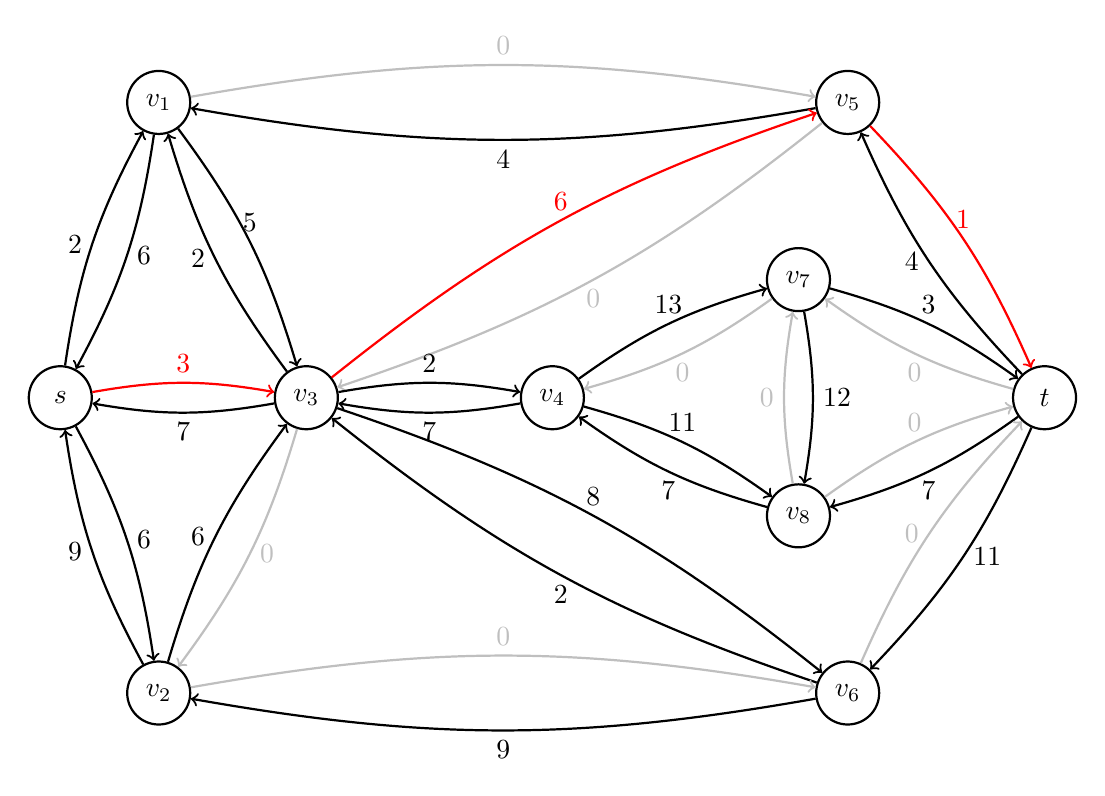
\begin{tikzpicture}[x=2.5cm, y=1.5cm]
		\begin{scope}[every node/.style={circle,thick,draw, minimum size=8mm}]
			\node (s) at (0,0) {$s$};
			\node (v1) at (0.5,2.5) {$v_1$};
			\node (v2) at (0.5,-2.5) {$v_2$};			
			\node (v3) at (1.25,0) {$v_3$};
			\node (v4) at (2.5,0) {$v_4$};
			\node (v5) at (4,2.5) {$v_5$};
			\node (v6) at (4,-2.5) {$v_6$};
			\node (v7) at (3.75,1) {$v_7$};
			\node (v8) at (3.75,-1) {$v_8$};
			\node (t) at (5,0) {$t$};
		\end{scope}
		\begin{scope}[every path/.style={thick,<-,bend right=10}]
			\path (s)  
			edge node[right] {6} (v1)
			edge node[left] {9} (v2)
			edge node[below] {7} (v3);
			\path (v1)
			edge node[left] {2} (v3)
			edge node[below] {4} (v5);
			\path (v2)
			edge [lightgray] node[right] {0} (v3)
			edge node[below] {9} (v6);
			\path (v3)
			edge [lightgray] node[below] {0} (v5)
			edge node[below] {7} (v4)
			edge node[below] {2} (v6);
			\path(v4)
			edge [lightgray] node[below] {0} (v7)
			edge node[below] {7} (v8);
			\path (v5)
			edge node[left] {4} (t);
			\path (v6)
			edge node[right] {11} (t);	
			\path[lightgray] (v7) 
			edge node[left] {0} (v8)
			edge node[below] {0} (t);
			\path (v8) 
			edge node[below] {7} (t);							
		\end{scope}
		\begin{scope}[every path/.style={thick,->, bend left=10}]
			\path (s)  
			edge node[left] {2} (v1)
			edge node[right] {6} (v2)
			edge [red] node[above] {3} (v3);
			
			\path (v1)
			edge node[above] {5} (v3)
			edge [lightgray] node[above] {0} (v5);
			\path (v2)
			edge node[left] {6} (v3)
			edge [lightgray] node[above] {0} (v6);
			\path (v3)
			edge [red] node[above] {6} (v5)
			edge node[above] {2} (v4)
			edge node[above] {8} (v6);
			\path (v4)
			edge node[above] {13} (v7)
			edge node[above] {11} (v8);
			\path (v5)
			edge [red] node[above] {1} (t);
			\path (v6)
			edge [lightgray] node[left] {0} (t);
			\path (v7) 
			edge node[right] {12} (v8)
			edge node[above] {3} (t);
			\path (v8) 
			edge [lightgray] node[above] {0} (t);
		\end{scope}
	\end{tikzpicture}
\end{minipage}
\begin{minipage}{.2\textwidth}
	\begin{tabular}{rr}
		\toprule
		what & value \\ \midrule
		$f(s,t)$ & 22 \\
		{\color{red}$\gamma$} & 1 \\
		\bottomrule
	\end{tabular}
\end{minipage}

\begin{minipage}{.8\textwidth}
	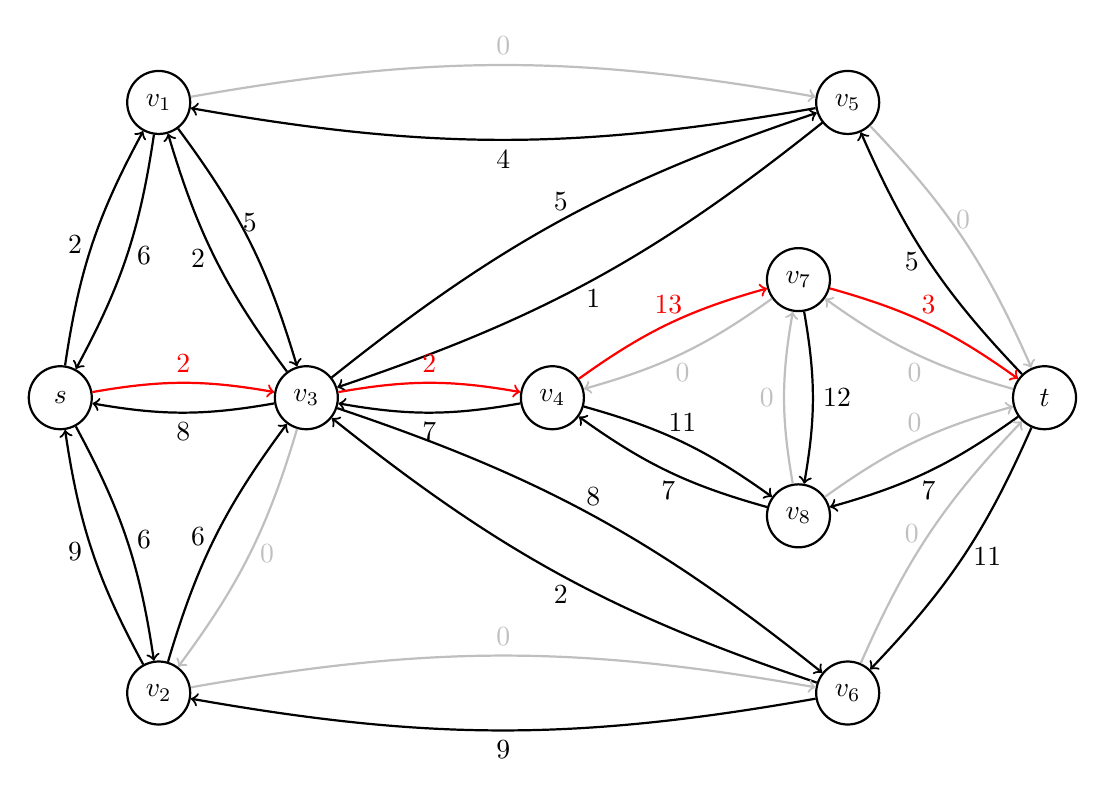
\begin{tikzpicture}[x=2.5cm, y=1.5cm]
		\begin{scope}[every node/.style={circle,thick,draw, minimum size=8mm}]
			\node (s) at (0,0) {$s$};
			\node (v1) at (0.5,2.5) {$v_1$};
			\node (v2) at (0.5,-2.5) {$v_2$};			
			\node (v3) at (1.25,0) {$v_3$};
			\node (v4) at (2.5,0) {$v_4$};
			\node (v5) at (4,2.5) {$v_5$};
			\node (v6) at (4,-2.5) {$v_6$};
			\node (v7) at (3.75,1) {$v_7$};
			\node (v8) at (3.75,-1) {$v_8$};
			\node (t) at (5,0) {$t$};
		\end{scope}
		\begin{scope}[every path/.style={thick,<-,bend right=10}]
			\path (s)  
			edge node[right] {6} (v1)
			edge node[left] {9} (v2)
			edge node[below] {8} (v3);
			\path (v1)
			edge node[left] {2} (v3)
			edge node[below] {4} (v5);
			\path (v2)
			edge [lightgray] node[right] {0} (v3)
			edge node[below] {9} (v6);
			\path (v3)
			edge node[below] {1} (v5)
			edge node[below] {7} (v4)
			edge node[below] {2} (v6);
			\path(v4)
			edge [lightgray] node[below] {0} (v7)
			edge node[below] {7} (v8);
			\path (v5)
			edge node[left] {5} (t);
			\path (v6)
			edge node[right] {11} (t);	
			\path[lightgray] (v7) 
			edge node[left] {0} (v8)
			edge node[below] {0} (t);
			\path (v8) 
			edge node[below] {7} (t);							
		\end{scope}
		\begin{scope}[every path/.style={thick,->, bend left=10}]
			\path (s)  
			edge node[left] {2} (v1)
			edge node[right] {6} (v2)
			edge [red] node[above] {2} (v3);
			
			\path (v1)
			edge node[above] {5} (v3)
			edge [lightgray] node[above] {0} (v5);
			\path (v2)
			edge node[left] {6} (v3)
			edge [lightgray] node[above] {0} (v6);
			\path (v3)
			edge node[above] {5} (v5)
			edge [red] node[above] {2} (v4)
			edge node[above] {8} (v6);
			\path (v4)
			edge [red] node[above] {13} (v7)
			edge node[above] {11} (v8);
			\path (v5)
			edge [lightgray] node[above] {0} (t);
			\path (v6)
			edge [lightgray] node[left] {0} (t);
			\path (v7) 
			edge node[right] {12} (v8)
			edge [red] node[above] {3} (t);
			\path (v8) 
			edge [lightgray] node[above] {0} (t);
		\end{scope}
	\end{tikzpicture}
\end{minipage}
\begin{minipage}{.2\textwidth}
	\begin{tabular}{rr}
		\toprule
		what & value \\ \midrule
		$f$ & 23 \\
		{\color{red}$\gamma$} & 2 \\
		\bottomrule
	\end{tabular}
\end{minipage}

\begin{minipage}{.8\textwidth}
	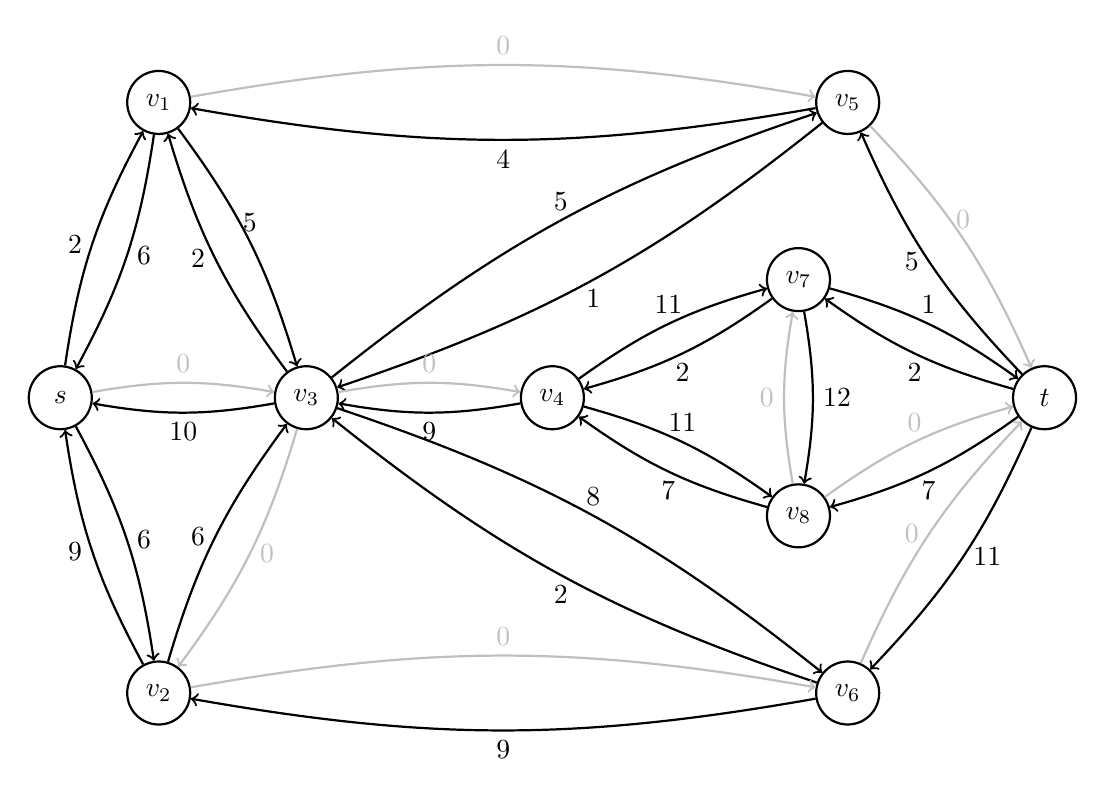
\begin{tikzpicture}[x=2.5cm, y=1.5cm]
		\begin{scope}[every node/.style={circle,thick,draw, minimum size=8mm}]
			\node (s) at (0,0) {$s$};
			\node (v1) at (0.5,2.5) {$v_1$};
			\node (v2) at (0.5,-2.5) {$v_2$};			
			\node (v3) at (1.25,0) {$v_3$};
			\node (v4) at (2.5,0) {$v_4$};
			\node (v5) at (4,2.5) {$v_5$};
			\node (v6) at (4,-2.5) {$v_6$};
			\node (v7) at (3.75,1) {$v_7$};
			\node (v8) at (3.75,-1) {$v_8$};
			\node (t) at (5,0) {$t$};
		\end{scope}
		\begin{scope}[every path/.style={thick,<-,bend right=10}]
			\path (s)  
			edge node[right] {6} (v1)
			edge node[left] {9} (v2)
			edge node[below] {10} (v3);
			\path (v1)
			edge node[left] {2} (v3)
			edge node[below] {4} (v5);
			\path (v2)
			edge [lightgray] node[right] {0} (v3)
			edge node[below] {9} (v6);
			\path (v3)
			edge node[below] {1} (v5)
			edge node[below] {9} (v4)
			edge node[below] {2} (v6);
			\path(v4)
			edge node[below] {2} (v7)
			edge node[below] {7} (v8);
			\path (v5)
			edge node[left] {5} (t);
			\path (v6)
			edge node[right] {11} (t);	
			\path (v7) 
			edge [lightgray] node[left] {0} (v8)
			edge node[below] {2} (t);
			\path (v8) 
			edge node[below] {7} (t);							
		\end{scope}
		\begin{scope}[every path/.style={thick,->, bend left=10}]
			\path (s)  
			edge node[left] {2} (v1)
			edge node[right] {6} (v2)
			edge [lightgray] node[above] {0} (v3);
			
			\path (v1)
			edge node[above] {5} (v3)
			edge [lightgray] node[above] {0} (v5);
			\path (v2)
			edge node[left] {6} (v3)
			edge [lightgray] node[above] {0} (v6);
			\path (v3)
			edge node[above] {5} (v5)
			edge [lightgray] node[above] {0} (v4)
			edge node[above] {8} (v6);
			\path (v4)
			edge node[above] {11} (v7)
			edge node[above] {11} (v8);
			\path (v5)
			edge [lightgray] node[above] {0} (t);
			\path (v6)
			edge [lightgray] node[left] {0} (t);
			\path (v7) 
			edge node[right] {12} (v8)
			edge node[above] {1} (t);
			\path (v8) 
			edge [lightgray] node[above] {0} (t);
		\end{scope}
	\end{tikzpicture}
\end{minipage}
\begin{minipage}{.2\textwidth}
	\begin{tabular}{rr}
		\toprule
		what & value \\ \midrule
		$f$ & 25 \\
		{\color{red}$\gamma$} & 0 \\
		\bottomrule
	\end{tabular}
\end{minipage}
There exists no augmenting $s$-$t$ path. The nodes reachable from $s$ are $v_1,v_2,v_3,v_5,v_6$.
\subsection{Show that the value of any $s$-$t$ flow $f$ is equal to the difference between the inflow into $t$ and the outflow at $t$, i.e.,$v(f) =f(\delta^-(t))-f(\delta^+(t))$}
By Lemma 4.3 a flow can be expressed via an $s$-$t$ cut as the following: $v(f)=f(\delta^+(C)) - f(\delta^-(C))$. Let $C$ be a cut where on one side are all vertices except $t$ ($C = V \setminus \{t\}$). The inflow into $t$ is precisely the outflow of the defined cut ($\delta^-(t) = \delta^+(C)$). Therefore the flow can be defined as $v(f) =f(\delta^-(t))-f(\delta^+(t))$.

\section{Problem 2: Flow through intermediate vertices}
\subsection{
Let $G= (V,A)$ be a directed graph with arc capacities $u:A\rightarrow\mathbb{Z}_{\geq0}$, and let $s_1,s_2,\ldots,s_l \in V$ be distinct. Assume that for every $i \in \{1,\ldots,l-1\}$, there is an $s_i-s_{i+1}$ flow $f_i$ with value $v(f_i)\geq k$ for some $k\in \mathbb{Z}_{\geq 0}$. Prove that there exists an $s_1$-$s_l$ flow $f$ with value $v(f)\geq k$.
}

if there exists a path $s_1$-$s_2$ with flow $f_1 \geq k$ and a path $s_2$-$s_3$ with flow $f_2\geq k$, there exists a path $s_1$-$s_3$ with a flow $f_{1,3} \geq k$. 
With this definition there exists an $s_1$-$s_l$ path with $f \geq k$.

\section{Problem 3: Max-flow min-cut via duality I}

\begin{equation}
	\begin{array}{llrcl}
		\max & \nu \\
		\text{s.t.} && \sum_{a\in\delta^+(v)}f_a - \sum_{a\in\delta^-(v)}f_a & = & \begin{cases}
			\nu &\text{if } v=s \\
			-\nu & \text{if } v=t \\
			0 & \text{if } v\in V \setminus \{s,t\}
			\end{cases} \\
		&& f_a & \leq & u_a \quad \forall a \in A \\
		&& f_a, v & \in & \mathbb{R}_{\geq 0}
	\end{array}
\label{eq:prob3_lp}
\end{equation}
\subsection{Prove that the optimal value of \autoref{eq:prob3_lp} equals the value of a maximum $s$-$t$ flow in $G$.}
To prove this, we need to show that the \autoref{eq:prob3_lp} is equal to the definition 4.1. (i) of the definition states the following: \textit{Capacity constraints: $f(a) \leq u(a) \quad \forall a \in A$}. This is precisely what the second constraint in the LP states. The (ii) part states the following: \textit{Balance constraints: for $v\in V$, $f(\delta^+(v)) - f(\delta^-(v)) \begin{cases}
=0 & \text{if } v \in V \setminus \{s,t\} \\
\geq 0 & \text{if } v = s \\
\leq 0 & \text{if } v = t
\end{cases}$}. There are three parts to prove. 

It's easy to see that $\sum_{a\in\delta^+(v)}f_a - \sum_{a\in\delta^-(v)}f_a = 0$ is equal to $f(\delta^+(v)) - f(\delta^-(v)) = 0$. 

$\nu$ is the value of the flow, so it corresponds to the outflow of $s$. Therefore the sum of all outflows of $s$ must equal $\nu$

With the same argument, the inflow for $t$ has to equal the value of $\nu$.

\subsection{Write down the dual of the linear program \autoref{eq:prob3_lp}, using variables $y_v$ for $v\in V$ and $z_a$ for $a\in A$.}

\begin{equation}
	\begin{array}{llrcl}
		\min & \sum_{a\in A} u_a z_a  \\
		\text{s.t.} 
	\end{array}
	\label{eq:prob3_lp}
\end{equation}
\end{document}